% One-page argument; figures are separate floats for manuscript placement.
\subsection{Why joint training acquires scale slowly}
\label{sec:scale-acquisition}

Can joint training acquire the scales needed for high precision?
After five million updates on mixed sine, joint Adam reaches relative error
$1.81\times10^{-3}$, versus $6.62\times10^{-7}$ on supplied features.
Its RMS relative slope reaches $0.0582$, compared with the supplied $1/4$;
GD acquires less scale (Figure~\ref{fig:scale-observation}). The preceding
accuracy results motivate explaining this slow population movement.

\paragraph{The surviving force.}
For squared loss $L=\frac12\|q_\theta-f\|^2$, splitting output into its
affine part and orthogonal remainder gives $\nabla L=R+F$. The
\emph{tracking gradient} $R$ measures departure from coarse equilibrium.
The \emph{effective fine gradient} $F$ combines the non-affine residual
gradient with the compensation needed to preserve coarse output.
In the audited GD regime, tracking is small; compensation remains within $F$.
We study the ensuing effective flow $\dot\theta=-F$ and account for
tracking and finite GD steps through explicit disturbance allowances.

\paragraph{Why weak force persists.}
Let $e_H$ be the non-affine residual, $J_H=D_\theta e_H$, and
$v=F/\|F\|$. Along effective flow,
\begin{equation}
\frac{d}{dt}\log\|F\|
=-\underbrace{\|J_Hv\|^2}_{\text{residual relaxation}}
+\underbrace{\kappa_H+\kappa_C}_{\text{geometry and compensation feedback}}.
\label{eq:scale-force-identity}
\end{equation}
Relaxation fits away the error driving the force; feedback changes
sensitivity to the remaining error. Small $F$ means weak residual coupling
after compensation. Rapid acquisition requires this coupling to strengthen.
On smooth step, force grows 2.19-fold while error remains near 49\%
(Figure~\ref{fig:scale-mechanism}): reinforcement occurs, but remains limited.
We bound its accumulation by $B_t$, using the population's second output
response weighted by residual and compensation norms.

\begin{theorem}[Slow scale acquisition, informal]
\label{thm:scale-informal}
Restart GD after tracking becomes small. Let $F_0$ and $E_0$ be the
restart effective gradient and non-affine residual norm, and $t=n\eta$.
If accumulated feedback is bounded by $B_t$, then, under the conditions in
Appendix~\ref{app:scale-theory},
\begin{align}
\|q_{\theta_n}-f\|^2
&\ge E_0^2-2t e^{2B_t}\|F_0\|^2-\Delta_{\mathrm{err}}(t),
\label{eq:scale-main-error}\\
\lambda_{\mathrm{RMS}}(t)
&\le\lambda_{\mathrm{RMS}}(0)
+\frac{h}{\sqrt W}t e^{B_t}\|F_0\|+\Delta_{\mathrm{scale}}(t).
\label{eq:scale-main-rms}
\end{align}
Here $\lambda_{\mathrm{RMS}}=h\|\gamma\|_2/\sqrt W$; $h$ is the
reference spacing. The allowances cover tracking and finite steps and
vanish for effective flow.
\end{theorem}

The proof bounds force amplification, then integrates force to bound
population travel and its square to bound output improvement.
A complementary theorem closes the mechanism: if population travel
produces limited additional reinforcement and accumulated force
concentration is controlled, weak force supplies too little movement
to amplify itself rapidly. Its finite-time condition and first-exit proof
are in Appendix~\ref{app:scale-loop}; parameters remain free to evolve.

\paragraph{Empirical check.}
The broader feedback condition covers all 46 sampled paths across 23
targets over 20k further updates. Six dense continuations over 100k further
updates give RMS growth bounds below $8\times10^{-4}$ and relative-error
floors above 39\%, with close GD/effective-flow agreement. The stronger
loop criterion passes all six shorter continuations and three longer ones
(Appendix~\ref{app:scale-experiments}). It explains a sufficient mechanism
for persistence; the broader theorem retains longer coverage.

% Review uses a separate float page. Place these two pairs near their
% discussion when integrating with the full manuscript.
\begin{figure}[p]
  \centering
  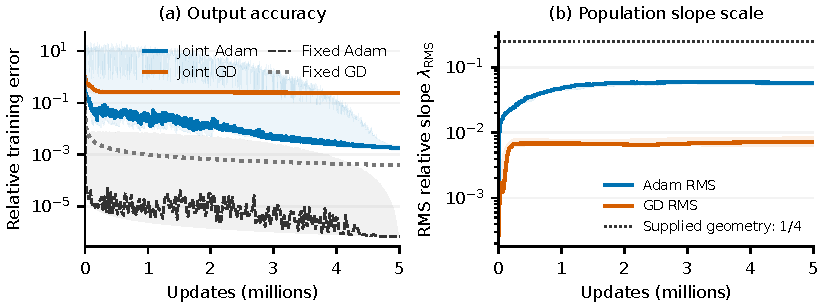
\includegraphics[width=\linewidth]{results/checkpoint_D_optimizers/expD34_readout_race/population_output/evidence/paper_latex_figures/joint_acquisition_rms.pdf}
  \caption{\textbf{Limited scale acquisition accompanies the precision gap.}
  Mixed sine, width 512, five paired seeds, five million full-batch updates.
  Left: relative training errors with trained readouts; fixed Adam/GD use
  uniform $\lambda=1/4$ features. Right: RMS relative slopes, $h=2/467$.
  Bands retain seed variation and within-bin extrema. Joint and fixed-Adam
  recipes use final-validation selection (Appendix~\ref{app:scale-experiments}).}
  \label{fig:scale-observation}
\end{figure}

\begin{figure}[p]
  \centering
  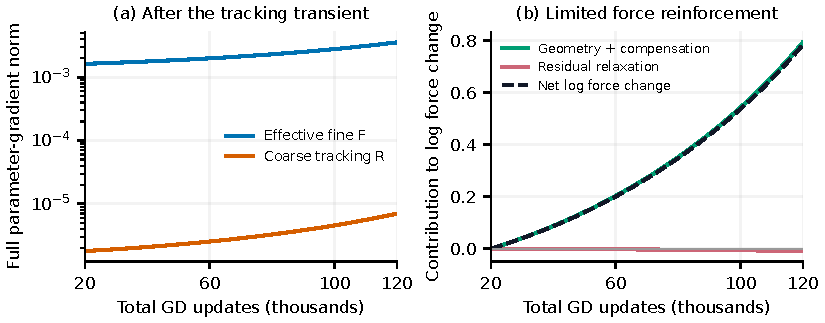
\includegraphics[width=\linewidth]{results/checkpoint_D_optimizers/expD34_readout_race/population_output/evidence/paper_latex_figures/tracking_and_reinforcement.pdf}
  \caption{\textbf{Weak effective force survives positive reinforcement.}
  Matched smooth-step continuations, width 705, from age 20k to 120k.
  Left: GD full-parameter gradient norms; tracking stays below 0.2\% of
  effective force at saved times. Right: cumulative terms
  in~\eqref{eq:scale-force-identity} along paired effective flow.
  Both axes use total GD updates with $\eta=0.002$; paired force norms
  differ by less than 0.08\%.}
  \label{fig:scale-mechanism}
\end{figure}

